\section{Workflow}
\label{sec:wokflow}

A typical workflow of charge transport simulations is depicted in \fig{workflow}. The first step is the simulation of an \slink{morphology}{atomistic morphology}, which is then partitioned on \slink{segments}{hopping sites}. The coordinates of the hopping sites are used to construct a list of pairs of molecules, or \slink{neighborlist}{neighbor list}. 

\begin{figure}[h]
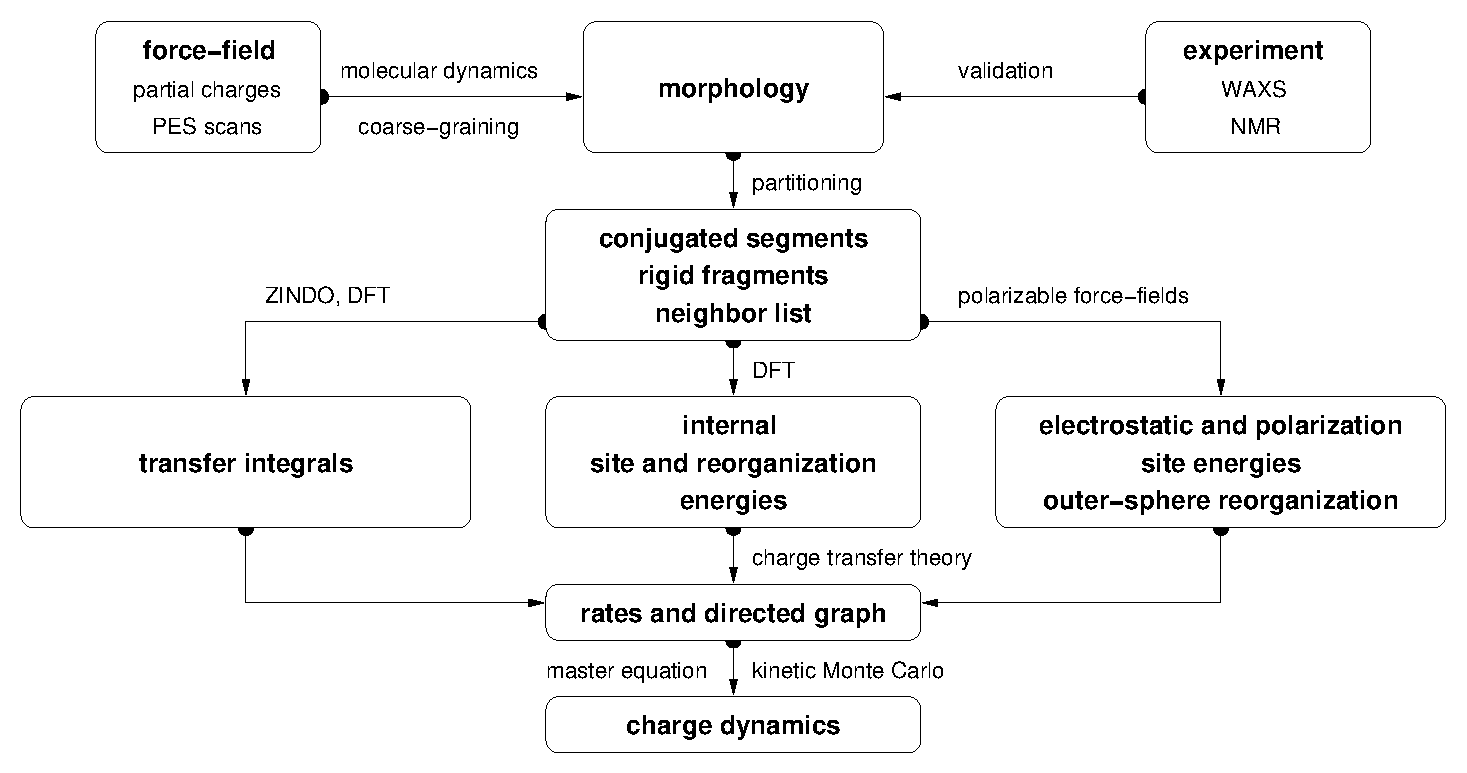
\includegraphics[width=\textwidth]{fig/workflow/workflow}
 \caption{%
   Workflow for microscopic simulations of charge transport.  %
   \label{fig:workflow}}
\end{figure}

For each pair an \slink{transfer_integrals}{electronic coupling element}, a \slink{reorganization}{reorganization energy}, a \slink{site_energies}{driving force}, and eventually the \slink{rates}{hopping rate} are evaluated. The neighbor list and hopping rates define a directed graph. The corresponding master equation is solved using the \slink{kmc}{kinetic Monte Carlo} method, which allows to explicitly monitor the charge dynamics in the system as well as to calculate time or ensemble averages of occupation probabilities, charge fluxes, correlation functions, and field-dependent mobilities.


\begin{figure}[p]
\includegraphics[width=\textwidth]{fig/workflow_practical/workflow_practical}
 \caption{%
   Workflow for microscopic simulations of charge transport including calls.  %
   \label{fig:workflow}}
\end{figure}


\tikzstyle{decision} = [diamond, draw, fill=blue!50]
\tikzstyle{line} = [draw, -stealth, thick]
\tikzstyle{elli}=[draw, ellipse, fill=red!50,minimum height=8mm, text width=5em ]
\tikzstyle{block} = [draw, rectangle, fill=blue!50, text width=\linewidth]
\tikzstyle{smallblock} = [draw, rectangle, fill=blue!50, text width=0.4\linewidth]
\begin{figure}
\centering
\newcommand{\vgap}{0.5cm}
\begin{footnotesize}
\noindent\begin{tikzpicture}
\node [block] (mapping) {{\bf Mapping}\\Converts and partitions atomistic \gromacs trajectory \vskip 0.1cm
{\noindent  \ctpmap \tpl \topology \trj \trajectory \seg \xmlcsg  \sql \sqlstate}
\vskip 0.1cm};

\node [block, below=\vgap of mapping] (nbl) {{\bf Neighbor list}\\Indentifies close molecular pairs between which charge transfer rates will be calculated \vskip 0.1cm
{\noindent  \ctprun \opt \xmloptions  \seg  \xmlsegments \sql  \sqlstate \exe  \calc{neighborlist}}
\vskip 0.1cm};


\node [block, below=\vgap of nbl] (site_energies) {{\bf Site energies}\\Calculates electrostatic and polarization contribution to site energies \vskip 0.1cm
{\noindent  \ctprun \opt \xmloptions  \sql  \sqlstate \exe  \calc{emultipole} } };

\node [block, below=\vgap of site_energies] (int_energies) {{\bf Internal site and reorganization energies}\\Imports internal site energy (IP, EA) and reorganization energies for charging and discharging to \sqlstate \vskip 0.1cm
{\noindent  \ctprun \opt \xmloptions  \sql  \sqlstate \exe  \calc{einternal} }
\vskip 0.1cm};


% above right=0.7cm and 4cm of A
\node[decision, below=\vgap of int_energies](decision1){Transfer integrals};

%\node (AuxNode01) [text width=6em, below of = decision1, node distance=7em ] {};

\node [smallblock, below left=\vgap of decision1] (DFT_TI) {{\bf Monomers with DFT}\\Calculate the relevant transport orbitals of monomers\\ prepare job file \vskip 0.1cm
{ \ctpparallel \opt \xmloptions \sql \sqlstate \exe \calc{edft} \job \wrt }
\vskip 0.1cm execute jobs \vskip 0.1cm
{ \ctpparallel \opt \xmloptions \sql \sqlstate \exe \calc{edft} \job \run }
};

\node [smallblock, below=\vgap of DFT_TI] (DFT_TI2) {{\bf Electronic coupling with DFT}\\Calculate electronic coupling elements for all pairs in the neighbor list \vskip 0.1cm
{ \ctpparallel \opt \xmloptions \sql \sqlstate \exe \calc{idft} \job `` \wrt \run \rd\'' }
\vskip 0.1cm};

\node [smallblock, below right=\vgap of decision1] (DFT_ZINDO) {{\bf Electronic coupling with ZINDO}\\Imports internal site energy (IP, EA) and reorganization energies for charging and discharging to \sqlstate \vskip 0.1cm
{\noindent  \ctprun \opt \xmloptions  \sql  \sqlstate \exe  \calc{einternal} }
\vskip 0.1cm};

\node (AuxNode01) [below=\vgap of DFT_TI2, xshift=0.25\linewidth] {};


\node [block, below=\vgap of DFT_TI2, xshift=0.275\linewidth] (outer_reorg) {{\bf Outersphere reorganization energies}\\Imports internal site energy (IP, EA) and reorganization energies for charging and discharging to \sqlstate \vskip 0.1cm
{\noindent  \ctprun \opt \xmloptions  \sql  \sqlstate \exe  \calc{outersphere} }
\vskip 0.1cm};

\node [block, below=\vgap of outer_reorg] (rates) {{\bf Charge transfer rates}\\Calculates rates for charge transfer among all pairs in the neighborlist \vskip 0.1cm
{\noindent \small \ctprun \opt \xmloptions \sql  \sqlstate \exe  \calc{rates} }
};

\node [block, below=\vgap of rates] (kmc) {{\bf Charge dynamics via kMC}\\Hopping of charge carriers simulated via kinetic Monte Carlo \vskip 0.1cm
{\noindent  \kmcrun \opt \xmloptions  \sql  \sqlstate \exe  \calc{kmcmultiple} }
};
%%
%(ClOp.west) -- ++(-0.2,0) -- ([yshift=0.5cm, xshift=-0.2cm] Pressure.north west) -|
%     ([xshift=-1cm]Sensor.south);
%    \draw[myarrow] (Ammeter.east) -- ++(0.2,0) -- ([yshift=0.5cm, xshift=0.2cm] Temperature.north east) -|
%     ([xshift=1cm]Sensor.south);

%\node [block, left of=mapping, xshift=-5em] (nbl) {Process 1};
%\node [elli, above of=mapping, yshift=5em] (user) {user};
%\node [block, right of=mapping, xshift=5em] (process2) {Process 2};
%\node[decision, below of=mapping, yshift=-5em](decision1){Process 1?};
%arrows
%\path [line] (user) -- (mapping);
\path [line] (mapping) -- (nbl);
\path [line] (nbl) -- (site_energies);
\path [line] (site_energies) -- (int_energies);
\path [line] (int_energies) -- (decision1);
\path [line] (DFT_TI) -- (DFT_TI2);
\path [line] (decision1) -| node[yshift=0.5em, xshift=1em] {DFT} (DFT_TI);
\path [line] (decision1) -| node[yshift=0.5em, xshift=-1em] {ZINDO} (DFT_ZINDO);
\path [line] (DFT_TI2) -- (outer_reorg);
\path [line] (DFT_ZINDO) -- (outer_reorg);
\path [line] (outer_reorg) -- (rates);
\path [line] (rates) -- (kmc);
\end{tikzpicture}


\end{footnotesize}
\caption{LALA}
\end{figure}

